\documentclass[twocolumn]{article}
\usepackage[utf8]{inputenc}
\usepackage[pdftex]{graphicx} %per poter inserire le figure
\usepackage{SIunits}
\usepackage{tabularx}
\usepackage{indentfirst}
\usepackage{verbatim} % multiline commenting
\usepackage{subfig}
\usepackage{caption}
\usepackage{footmisc} % to \ref to footnotes
\usepackage{lipsum}
\usepackage{eucal}
\usepackage{eso-pic}
\usepackage{url}
\usepackage{bm}
\usepackage{balance}
\usepackage{afterpage}
\usepackage{parskip}
\usepackage{listings}
\usepackage{multicol}
\setlength{\columnsep}{1cm}
\usepackage{fancyhdr}
\usepackage{textcomp}
\usepackage{multicol}
\usepackage{multirow}
\usepackage{subfiles}
\usepackage{microtype}
\usepackage{adjustbox}
\usepackage{amsmath}
\usepackage{setspace}
\usepackage{wrapfig}
\usepackage{float}
\usepackage{array}
\usepackage{color}
\usepackage[toc,page]{appendix}
\usepackage{hyperref}
\usepackage{colortbl}
\usepackage{bbold}
\usepackage{booktabs} %linee tabelle
\usepackage[labelfont=bf,size=small]{caption} %didascalie
\usepackage[backend=biber]{biblatex}

\addbibresource{mybib.bib}   %file della bibliografia

\pagestyle{fancy} 

\newcommand{\gio}[1]{\textcolor{blue}{\textit{#1}}}
\newcommand{\mean}[1]{\left\langle #1 \right\rangle}

\definecolor{graytext}{HTML}{414141}
\definecolor{linkcolor}{rgb}{0,0,0.65} %hyperlink
\definecolor{linescolor}{rgb}{0.65,0.16,0.16}
\definecolor{cool}{RGB}{49,54,149}
\definecolor{hot}{RGB}{165,0,38}

\usepackage{fancyhdr} 

\pagestyle{fancyplain}
\fancyhf{}
\lhead{\ifnum\value{section}>0\nouppercase{\textbf{\leftmark}\fi}}
\rhead{De Bei, Lo Presti Piccolo, Piccolo}
\chead{}

\fancyfoot[R]{Page \thepage}
\fancyfoot[L]{\textit{Nanofabrication, Characterization and Modelling of Colloidal Au Nanoparticles}}

\renewcommand{\headrulewidth}{0.2pt}
\renewcommand{\footrulewidth}{0.1pt}
\setlength\parindent{9pt} % To adjust the indentation

\title{}
\author{}
\date{}

\begin{document}

\thispagestyle{fancy}
\subfile{header.tex}
\thispagestyle{empty}

%\clearpage
\tableofcontents

\noindent\makebox[\linewidth]{\color{linescolor} \rule[-0.2cm]{0.85\paperwidth}{1pt}}
\noindent\makebox[\linewidth]{\color{linescolor} \rule[0.3cm]{0.85\paperwidth}{1.2 pt}}
%\pagebreak[4]

%\clearpage

\begin{multicols}{2}
\section{Introduction}
\noindent
Nanoparticle research has greatly expanded over the past decades. 
In particular, a major effort was put in the study and in the control of the shape and of the size of nanoparticles because of their influence over the electro-magnetic and optical properties of the nanoparticles themselves.

Among noble metal nanoparticles, the Gold nanoparticles are of special interest due to their prominent optical resonance in the visible range.

The Au nanoparticles' interaction with light is strongly dictated by the environment surrounding them, by their size and by their physical dimensions. Oscillating electric fields of a light ray propagating near a colloidal nanoparticle interact with the free electrons causing an oscillation of electron charge that can be in resonance with the frequency of visible light. These resonant oscillations are known as surface plasmons. 

The aim of this work is to describe and characterize colloidal spherical gold nanoparticles. 

In the first part of this paper we will illustrate the main steps of the synthesis of the Au nanoparticles by means of the \textit{Turkevich method} (\textbf{Section \ref{sec:synthesis}}). 

After the synthesis we obtained the optical spectrum of the gold nanoparticles in the Vis-NIR range using a JASCO V670 spectrophotometer in order to simulate the absorption line, to obtain the Mie extinction cross-section by means of the Mie theory in the dipolar approximation and to compute the size-corrected experimental dielectric function of Au (\textbf{Section \ref{sec:optic_char}}). 

The optical analysis of the gold nanoparticles allowed us to obtain informations on the size of the nanoparticles, on their concentration and on the refractive index of the medium.

We performed then independent measurements on the average size of spherical gold nanoparticles using the Grazing incidence X-Ray Diffraction (XRD): we estimated the diffraction of X-rays photons, coming from \(\text{Cu}_{k_\alpha}\), forming an angle of \(2\theta\) with respect to the incoming beam (\textbf{Section \ref{sec:XRD}}).

In the end, in \textbf{Section \ref{sec:SEM}}, we used a scanning electron microscope (SEM) to perform a statistical size distribution of the system, while \textbf{Section \ref{sec:conclusions}} summarizes the results of our work.

\newpage

\section{Synthesis of Au nanoparticles}
\label{sec:synthesis}
\noindent
Colloidal spherical gold nanoparticles can be synthesized via the Turkevich method: gold atoms are decomposed from a gold acid precursor forming a supersaturated solution and thus initiating the nucleation of the nanoparticles aggregating and growing under controlled constant temperature \cite{Kimling2006}.

This method allowed us to synthesize nanoparticles of the order of $5 \div 20 \,\nano\meter$ of diameters. \gio{non so se è proprio vero ma, forse si può togleire questa frase lol}

\subsection{Turkevich method}
The main steps which determine the Turkevich method can be summed up as follows:

\begin{enumerate}
    \item Pour in a beaker 9.5 mL of gold hydroclorate solution (HAuCl$_4$);
    \item Cover the beaker with a watch glass;
    \item Suspend the beaker in the crystallizer filled with normal water on the hot plate and rise the temperature up to 100\degreecelsius;
    \item Activate the stirrer in order to obtain an homogeneous distribution of temperature and concentration;
    \item Heat the sodium citrate solution (Na$_3$C$_6$H$_5$O$_7$) up to 100\degreecelsius;
    \item When both solutions are at 100 °C, add 0.5 mL of the Na$_3$C$_6$H$_5$O$_7$ solution to the beaker, which will decomposes the precursor by redox reduction in order to reduce gold atoms to metallic gold. The citrate concentration is chosen to prevent the formation of big structures;
    \item Wait 15 minutes with the stirrer on and at 100\degreecelsius.
\end{enumerate}

\noindent
The result we obtained can be seen in \textbf{Figure \ref{fig:sample}}.

\begin{figure}[H]
    \centering
    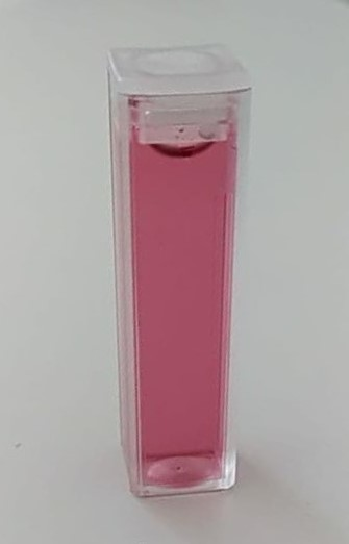
\includegraphics[width=0.5\linewidth]{image/data/turkevich.pdf}
    \caption{Sample of colloidal Au nanoparticles we obtained in the laboratory using the Turkevich method.}
    \label{fig:sample}
\end{figure}

\section{Optical Characterization}
\label{sec:optic_char}
\noindent
In order to acquire the optical spectrum of the colloidal Au nanoparticles we used a JASCO double beam spectrophotometer, which shines light in a continuous spectrum in the Vis-NIR range ($300\div 2700\, \nano\meter $).

To verify the presence of the localized surface plasmon resonance (LSPR) we acquired the absorbance spectrum: the spectrophotometer shoots on the sample a single wavelength at a time which is selected by a monocromator and then the same procedure is repeated for a second beam, which provides a baseline. At this point the transmittance $T$ is measured and then converted, using the \textit{Lambert-Beer} equation (\textbf{Equation \ref{eq:absorbance}}), into absorbance data $A$: 

\begin{equation}
    A:=\log_{10}\frac{1}{T}=\log_{10}(e)z \sigma_{ext} \rho
    \label{eq:absorbance}
\end{equation}

\noindent
where $z=1\, cm$ is the length of the sample, $\sigma_{ext}$ is the Mie extinction cross section and $\rho$ is the density of the nanoparticles.

The experimental data we obtained are plotted in \textbf{Figure \ref{fig:exp_data}}. As we can see, the spectrum exhibits a resonant behavior and the data near the peak can be used to estimate the properties of the system.

\begin{figure}[H]
    \centering
    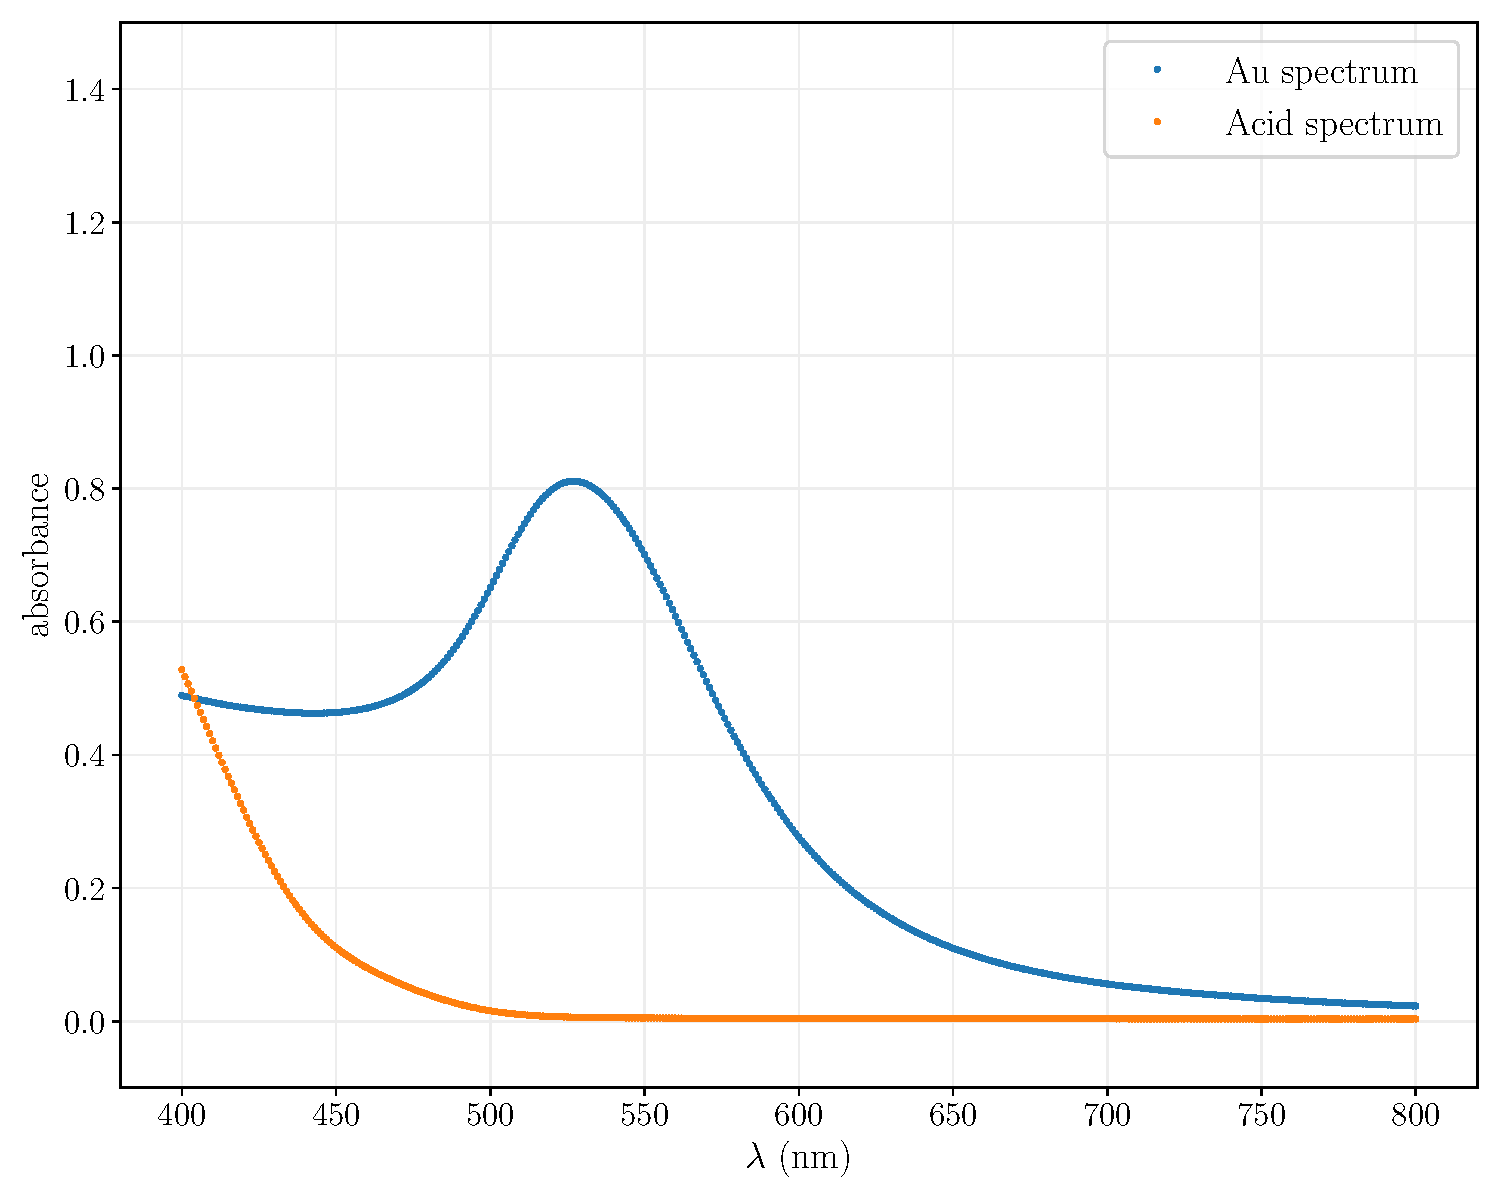
\includegraphics[width=\linewidth]{image/data/exp_data.pdf}
    \caption{Experimental spectra: in blue is plotted the Gold nanoparticle experimental spectrum, while in orange the acid spectrum.}
    \label{fig:exp_data}
\end{figure}

The label \textit{Acid spectrum} of \textbf{Figure \ref{fig:exp_data}} refers to the fact that in the first place we measured the optical spectrum of the medium in which nanoparticles were immersed, (which was water and tetrachloroauric acid),  and then we acquired the gold
nanoparticle solution spectrum (\textit{Au spectrum} label).

The following optical analysis has been performed in the $400 \div 800\,\nano\meter$ range.

\subsection{Model}
In order to apply the Mie theory in the dipolar approximation to the collected experimental data and in order to compute the extinction cross section we assumed some hypothesis on our physical system: first of all we supposed that the radius of the Au nanoparticles was much smaller with respect to the incident wavelengths ($R\ll \lambda$) and that the medium dielectric function was real ($\epsilon_m(\omega) \in \mathbb{R}$: non-absorbing matrix hypothesis). 

Furthermore, we supposed that the nanoparticles had spherical shape, that the system was monodispersed with respect to the particle radius and that the gold nanoparticles had a non real and size-dependent dielectric function $\epsilon(\omega,R) = \epsilon_1(\omega,R) +i\epsilon_2(\omega,R)$\footnote{In first approximation it is possible to assume that the dielectric function can be equal to the one computed by Johnson and Christy in \cite{Johnson1972}, where $\epsilon(\omega) = \epsilon_1(\omega) +i\epsilon_2(\omega)$, see \textbf{Figure \ref{fig:size_correction}}. In addition, $\omega=c/\lambda$ and $c$ is the speed of light.}, described by the following equation:

    \begin{small}
    \begin{equation*}
    \begin{split}
       \epsilon(\omega,R) & = \epsilon(\omega,\infty) + \omega_P^2 \left(\frac{1}{\omega^2+\Gamma_{bulk}^2}-\frac{1}{\omega^2+ \Gamma(R)^2}\right) \\ 
     & -i\frac{\omega_P^2}{\omega} \left(\frac{\Gamma_{bulk}}{\omega^2+\Gamma_{bulk}^2}-\frac{\Gamma(R)}{\omega^2+ \Gamma(R)^2}\right)
      \end{split}
      \label{eq:epsilon}
    \end{equation*}
    \end{small}

\noindent
where $\epsilon(\omega, \infty)$ is the bulk dielectric function, $\omega_P$ is the plasmon frequency of bulk gold and $\Gamma$ is the typical damping time for the electrons.\\

\noindent
In particular, according to the Drude model, 

\[\Gamma(R)=\Gamma_{bulk}+k \frac{v_{F}}{R}\]

\noindent
where $k=\pi/4$ in the assumption of spherical nanoparticles, $v_F$ is the Fermi velocity for gold electrons, $R$ is the nanoparticle's radius, $\Gamma(R)$ is the size-dependent electrons relaxation frequency and $\Gamma_{bulk}$ is the relaxation frequency in bulk gold. 

In \textbf{Table \ref{tab:bulk_const}} we report the bulk constants of gold used for this work. 

\begin{table}[H]
    \centering
    \caption{Bulk constants of gold at room temperature.}
    \begin{tabular}{ccc}
    \toprule
      \bm{$\omega_p$}  \cite{Kittel2004}  & \bm{$\Gamma_{bulk}$}  \cite{Johnson1972} & \bm{$v_{F}$} \cite{Ashcroft76} \\
    \midrule
      $1.38 \cdot 10^{16} \,\text{Hz} $   & $1.08 \cdot 10^{14} \,\text{Hz}$ & $1.40 \cdot 10^6 \, \meter/\text{s}$ \\
    \bottomrule
    \end{tabular}
    \label{tab:bulk_const}
\end{table}

\noindent
In order to obtain the size-dependent dielectric function equation we had to apply a semi-classical correction: from the Drude model for the electrons we can derive that
$$
\begin{array}{l}
\epsilon_{1}(\omega, R)=\epsilon_{1}(\infty)+\omega_{p}^{2}\left(\frac{1}{\omega^{2}+\Gamma_{bulk}^{2}}-\frac{1}{\omega^{2}+\Gamma(R)^{2}}\right) \\
\epsilon_{2}(\omega, R)=\epsilon_{2}(\infty)-\frac{\omega_{p}^{2}}{\omega}\left(\frac{\Gamma_{bulk}}{\omega^{2}+\Gamma_{bulk}^{2}}-\frac{\Gamma(R)}{\omega^{2}+\Gamma(R)^{2}}\right)
\end{array}
$$

\noindent
We can observe the effects of the size correction of the dielectric function in \textbf{Figure \ref{fig:size_correction}} for different values of the radius. With the plot label \textit{Johnson and Christy} we refer to non size corrected values of the dielectric function.

Using the second part of \textbf{Equation \ref{eq:absorbance}} we can express the absorbance $A$ as a function of the Mie extinction cross section as follows.

\noindent
Assuming a quasi-static field approximation and given that (\cite{Kimling2006})
\begin{equation}
\sigma_{e x t}=9 \frac{\omega}{c} \epsilon_{m}{ }^{3 / 2} {V} \frac{\epsilon_{2}}{\left(\epsilon_{1}+2 \epsilon_{m}\right)^{2}+\left(\epsilon_{2}\right)^{2}}
\end{equation}

\noindent
where $V$ is the nanoparticles' volume, we can use \textbf{Equation \ref{eq:absorbance}} and the spherical nanoparticles approximation to write $A$ as:

\begin{equation}
    A=K\epsilon_m^{3/2}R^3\rho\omega\frac{\epsilon_2}{(\epsilon_1 + 2\epsilon_m)^2 + (\epsilon_2)^2}
    \label{eq:ass}
\end{equation}
with $K=\log_{10}(e)\frac{9}{c}\frac{4\pi}{3}z$.

\end{multicols}

\begin{figure}[H]
    \begin{minipage}[l]{1.0\columnwidth}
    \centering
    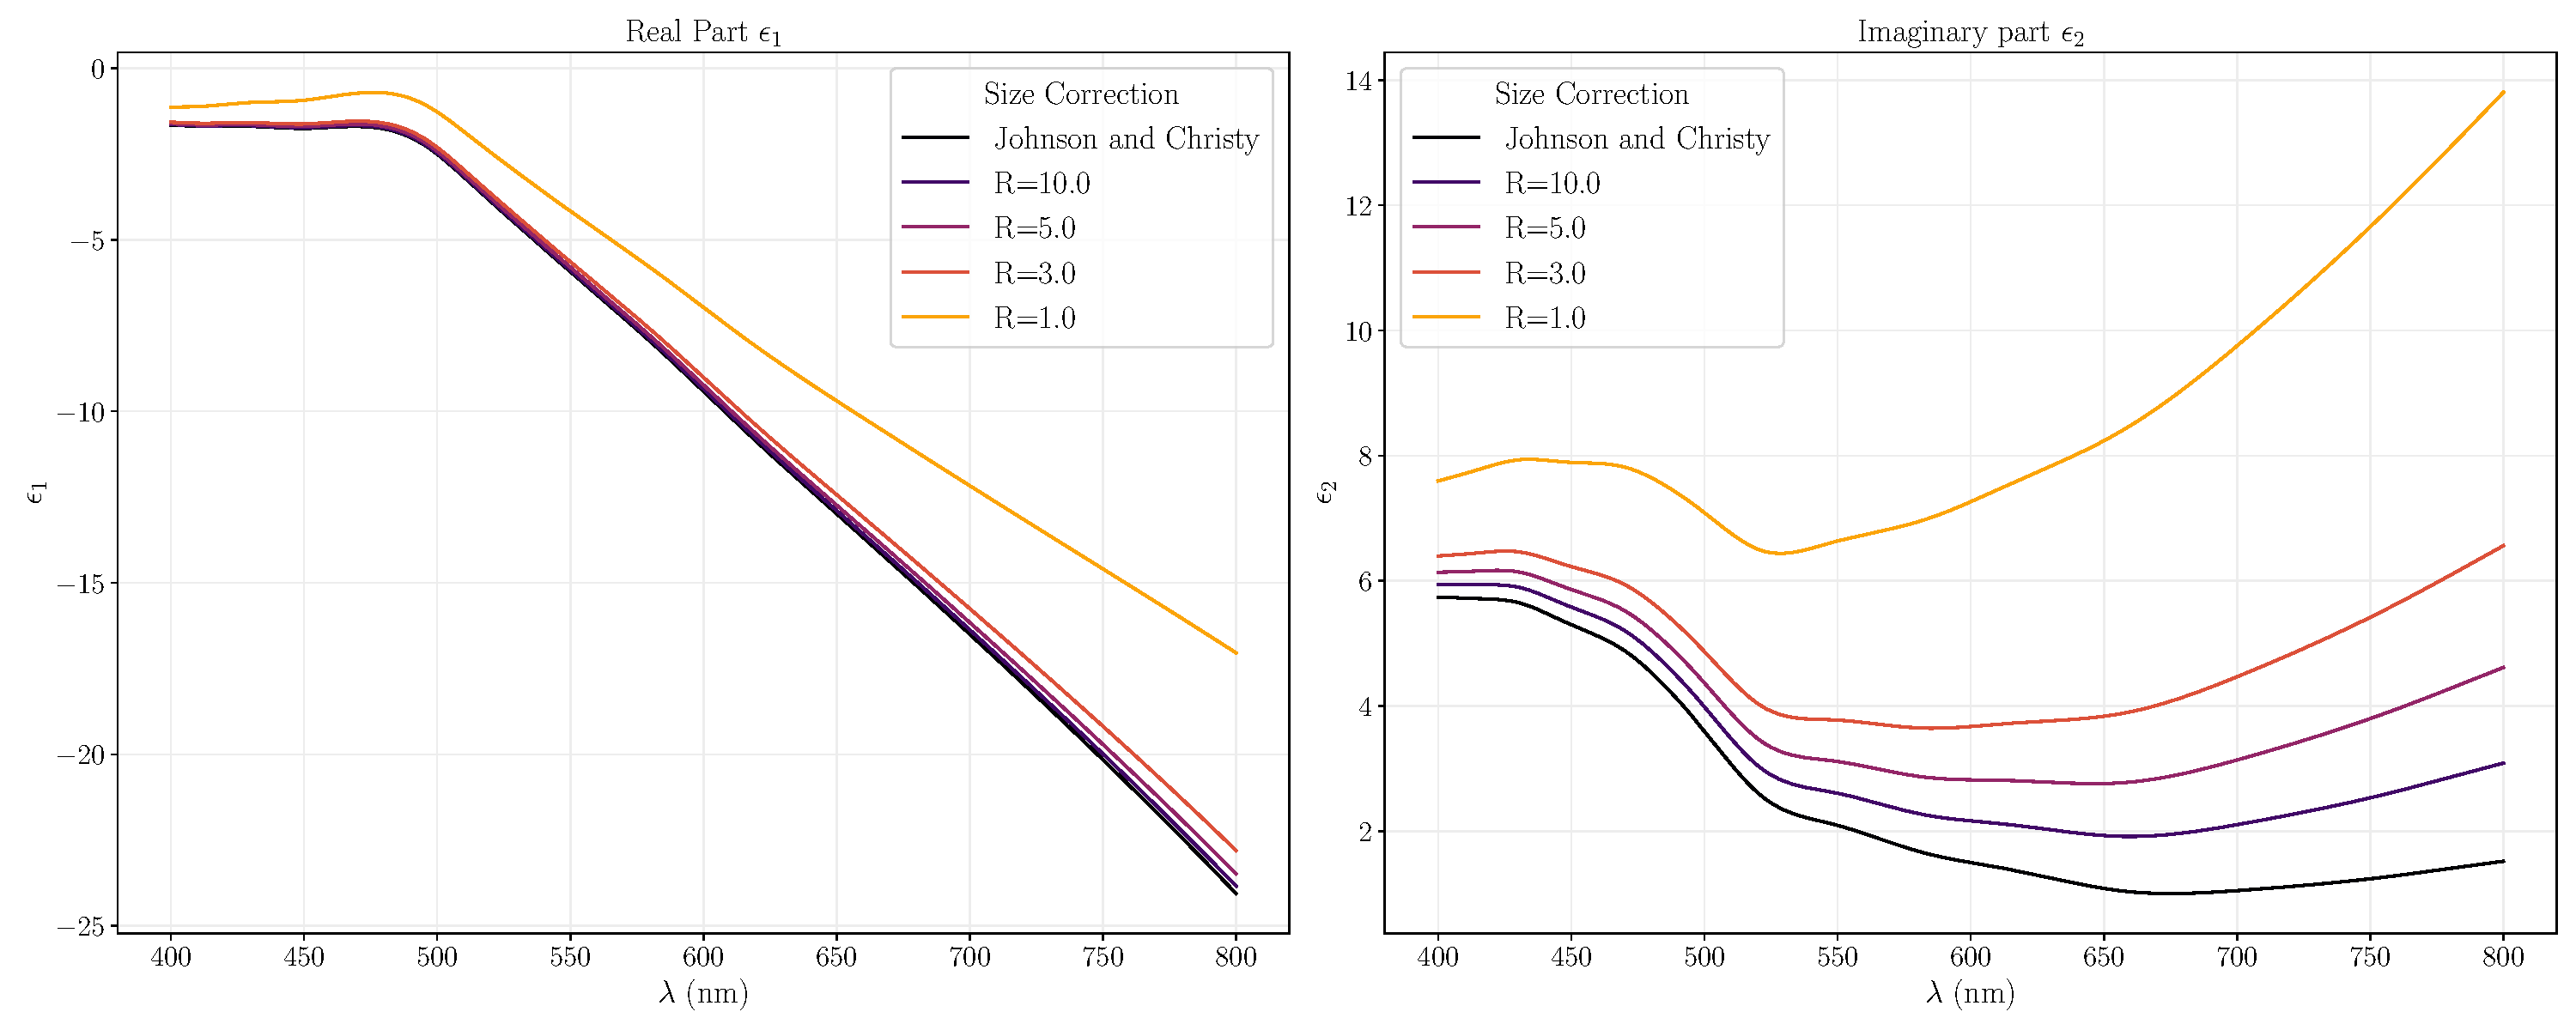
\includegraphics[width=\textwidth]{image/data/size_correction.pdf}
    \caption{Size correction of the dielectric function for different values of the radius. Johnson and Christhy label refers to non size corrected dielectric values.}
    \label{fig:size_correction}
    \end{minipage}
\end{figure}

\begin{multicols}{2}

Due to the presence of the $R^3\rho$ term in \textbf{Equation \ref{eq:ass}}, we have performed the optical analysis of the colloidal Au nanoparticles using from the beginning the size-dependent equation for the dielectric function i.e. using $\epsilon_1(\omega,R)$ and $\epsilon_2(\omega,R)$.

At this point we can model our system by varying its three free parameters ($\epsilon_m, \rho, R$). 

In order to find the best-fit parameters, we began our analysis by varying $R$ and by keeping $\rho$ and $\epsilon_m$ constant obtaining the fit for the couple ($R,\rho$). 

Then, we estimated the stability basin of the best fit result computing the minimized $\chi^2$, i.e. by computing:
\begin{equation}
        {\min}_{R,\rho} \left\{\chi^2 (R,\rho) \right\} =\min_{R,\rho} \left(\frac{A_{exp}-A_{sim}}{\sigma_{A_{exp}}}\right)^2 
\end{equation}
%\noindent
where $\sigma_{A_{exp}}={A_{exp}}^{-1}$ is the error of the experimental data of the absorbance (i.e. $A_{exp}$), while $A_{sim}$ is the simulated absorbance.%\footnote{We choose this value for the error in order to obtain a better agreement between data and simulation by giving a different weight to the spectrum values.}

From the first part of the optical analysis we were able to obtain the best value for $\rho$, namely $\rho^*$, by minimizing the $\chi^2$ function.

We proceeded then by repeating the steps previously described by fixing the value of the nanoparticles' density to be $\rho\overset{!}{=}\rho^*$. Then, by varying and fitting $R$ and $\epsilon_m$ and by minimizing the $\chi^2$ function with respect to ($R,\epsilon_m$), we obtained the last two best-fit parameters $R^*$ and $\epsilon_m^*$.

\subsection{Results}
\label{sec:risultati}

In this section we report the results obtained in the analysis presented in \textbf{Section \ref{sec:optic_char}.1}.
In the first place we verified the validity of the non-interacting nanoparticles assumption by computing the filling fraction $f=\rho^* V$. This approximation is valid if $f\ll 1 $ and since we estimated the filling fractions as
\[f=2.16\cdot 10^{-6}\]
we can state that the contribution due to interacting nanoparticles is negligible.

In order to simulate the spectrum of the couple $(R,\rho)$ we fixed the medium dielectric constant to be equal to 
\[\epsilon_m=n_{water}^2=1.33^2\]

\noindent
namely to be equal to the square of the refractive index of water.

The simulated spectrum of the couple ($R,\rho$) is reported in \textbf{Figure \ref{fig:r_rho}a}. As shown in the plot, the agreement between the experimental and the simulated data is not good, especially for the lower wavelengths.

In \textbf{Figure \ref{fig:r_rho}b} is instead reported the $\chi^2$ map as a function of $R$ and $\rho$ in order to verify the stability of the fit parameters. We can observe that we do not get an unique minimum for the $\chi^2$: the presence of an elongated region with low $\chi^2$ may be probably due to the correlation between $R$ and $\rho$ in the absorbance formula reported in \textbf{Equation \ref{eq:ass}}.

\textbf{Figure \ref{fig:r_epsm}a} reports instead the fit between $R$ and $\epsilon_m$ after that we had set 

\[\rho \overset{!}{=} \rho^*=9.909\cdot10^{-9}\,\nano\meter^{-3}.\]

\noindent
The second plot shows that the agreement with the experimental spectrum is improved, even if the fit remains quite poor in the $\lambda \in [400:475]\, \nano\meter$ region due to the high value of the absorbance.

The \( (R,\epsilon_m) \) plot of the $\chi^2$ function, presented in \textbf{Figure \ref{fig:r_epsm}b}, shows that the stability region is more focused, inducing an $\epsilon_m^*$ value which is probably more precise with respect to $\rho^*$.

\noindent
To sum up, the best values for the three parameters ($R$, $\rho$, $\epsilon_m$) are:
\begin{align*}
    R^* &= (4\pm 1)\, \text{nm}\\
    \rho^* &= (10 \pm 3)\cdot 10^{-9} \text{nm}^{-3} \\
    \epsilon_m^* &= 2.1 \pm 0.3
\end{align*}

\noindent
The uncertainties associated to these values are coherent with the two $\chi^2$ maps but they result in very high error values (in particular the one associated to the nanoparticles' density), preventing the best fit parameters ($R^*, \rho^*, \epsilon_m^*$) to be good reliable values. 

We can perform a compatibility test between $\epsilon_m^*$ and $n_{water}^2$, which can be estimated as $\Tilde{\lambda}_{\epsilon_m}=1.1$, which shows a good (but not optimal) compatibility between our estimate and the true value of the dielectric constant of the medium.

Our analysis could have been improved by performing a Cauchy analysis on $\epsilon_m$. In this paper we assumed that the value of the dielectric constant of the medium was not influenced by $\lambda$ but actually the refractive index of the medium can depend on the wavelength and this behaviour can be described by the Cauchy law
\begin{equation*}
\epsilon_{m}(\lambda)=n_{m}(\lambda)^{2}=\left(n_{water}+\frac{B}{\lambda^{2}}\right)^{2}
\end{equation*}
and by introducing a new free parameter $B\overset{!}{\geq} 0$\,\footnote{We impose $B\geq 0$ because the refractive index decreases moving towards the infrared range of wavelengths.}.


\end{multicols}
\newpage
\begin{figure}[H]
\centering
\subfloat[][{Simulated spectrum obtained by varying the parameters ($R,\rho$) and fit with the experimental data.}]
{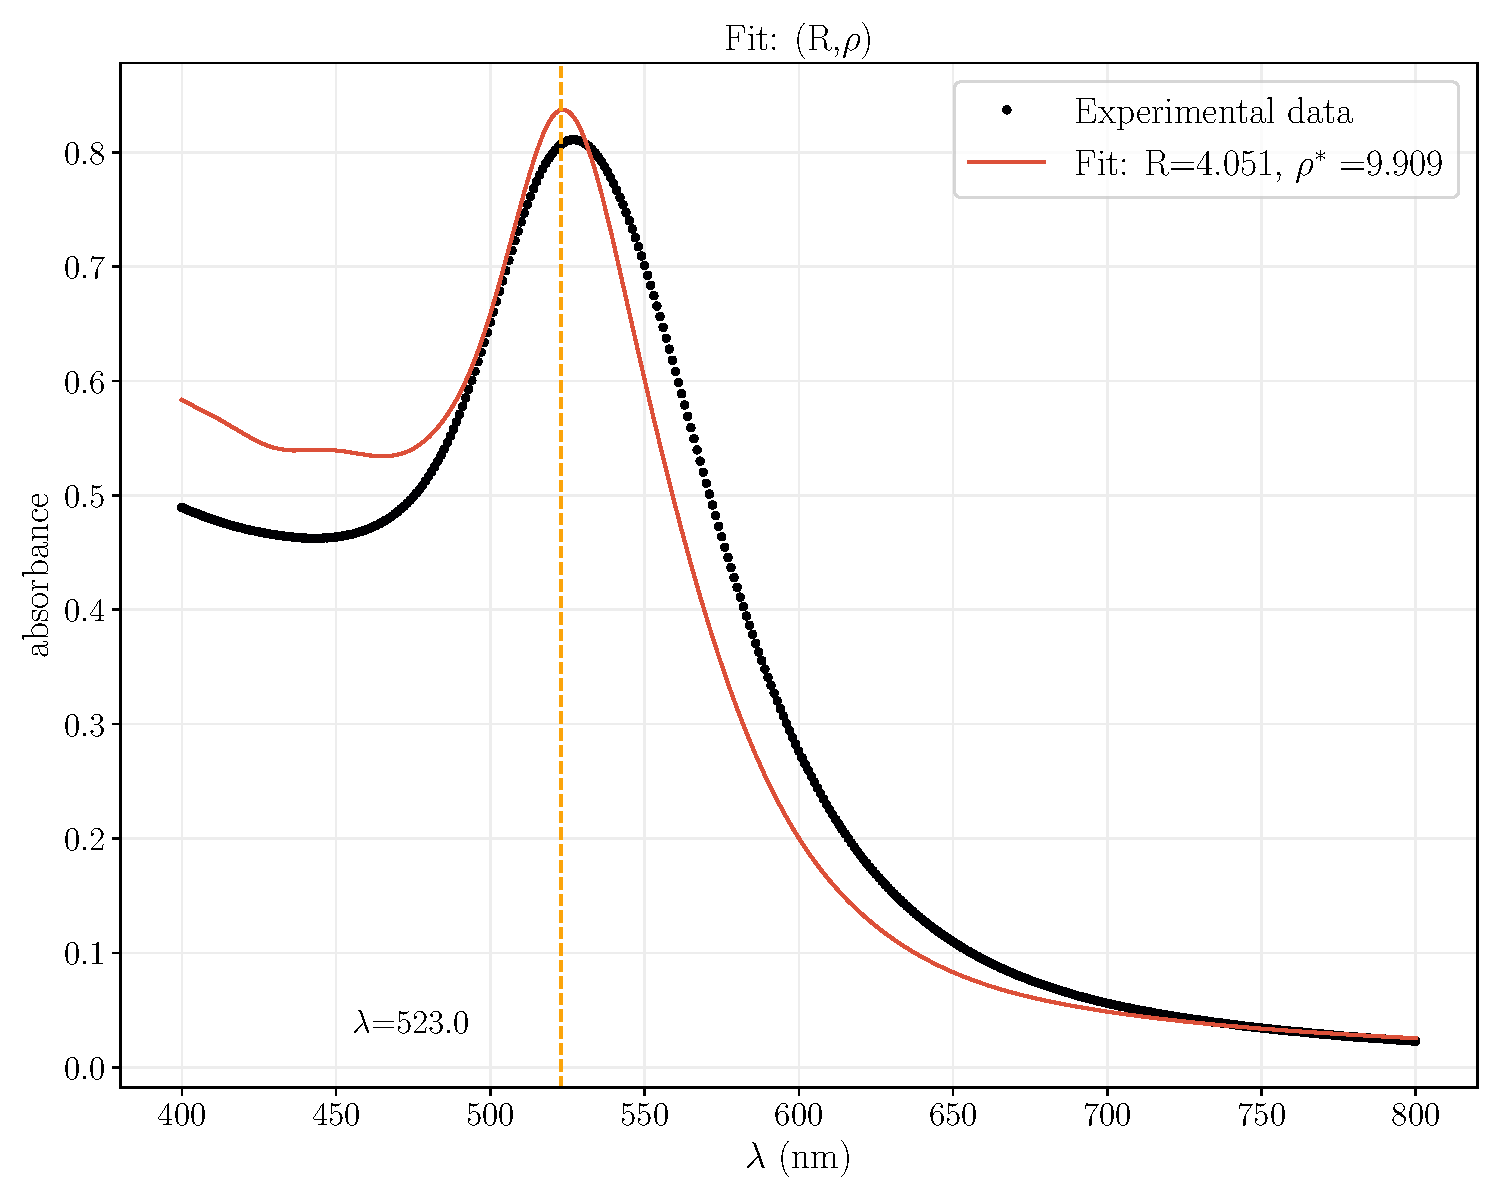
\includegraphics[width=.5\textwidth]{image/data/1_fit.pdf}} 
\subfloat[][{Map of the $\chi^2$ function for ($R,\rho$).}]
{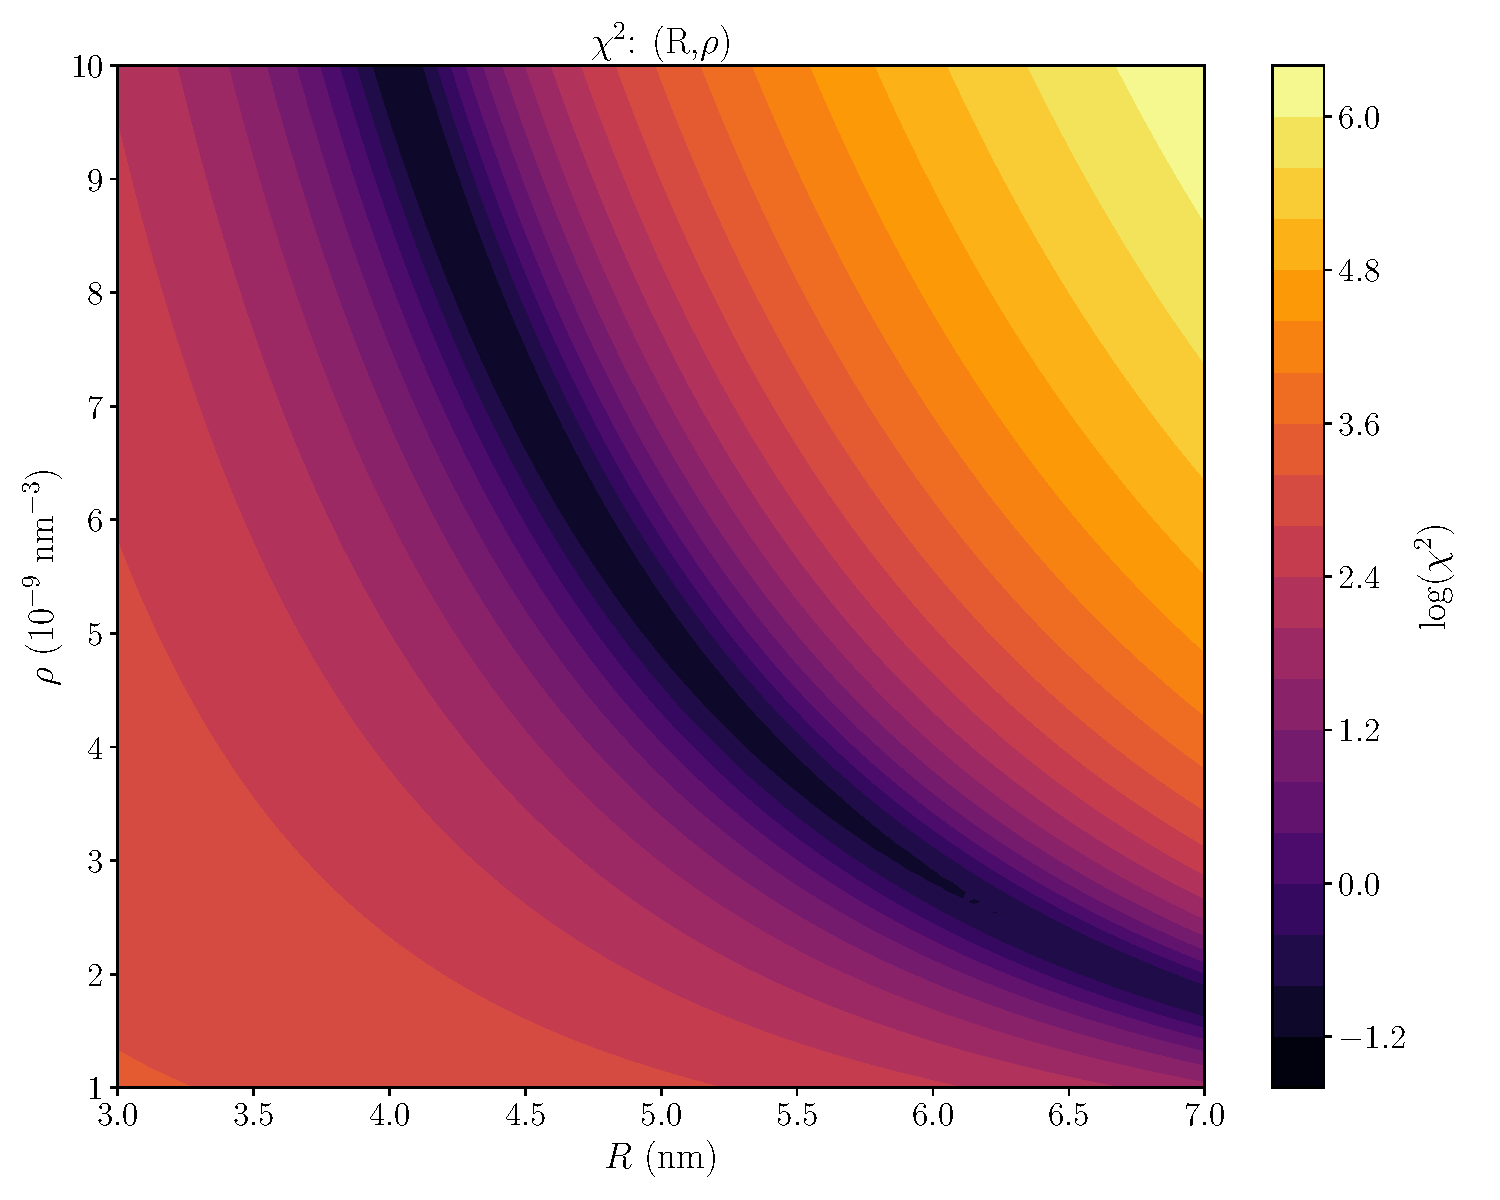
\includegraphics[width=.5\textwidth]{image/data/1_chisquare.pdf}} \\
\caption{Simulation, fit and plot of the $\chi^2$ function for the ($R,\rho$) couple.}
\label{fig:r_rho}
\end{figure}

\begin{figure}[H]
\centering
\subfloat[][{Simulated spectrum obtained by varying the parameters ($R,\epsilon_m$) and fit with the experimental data.}]
{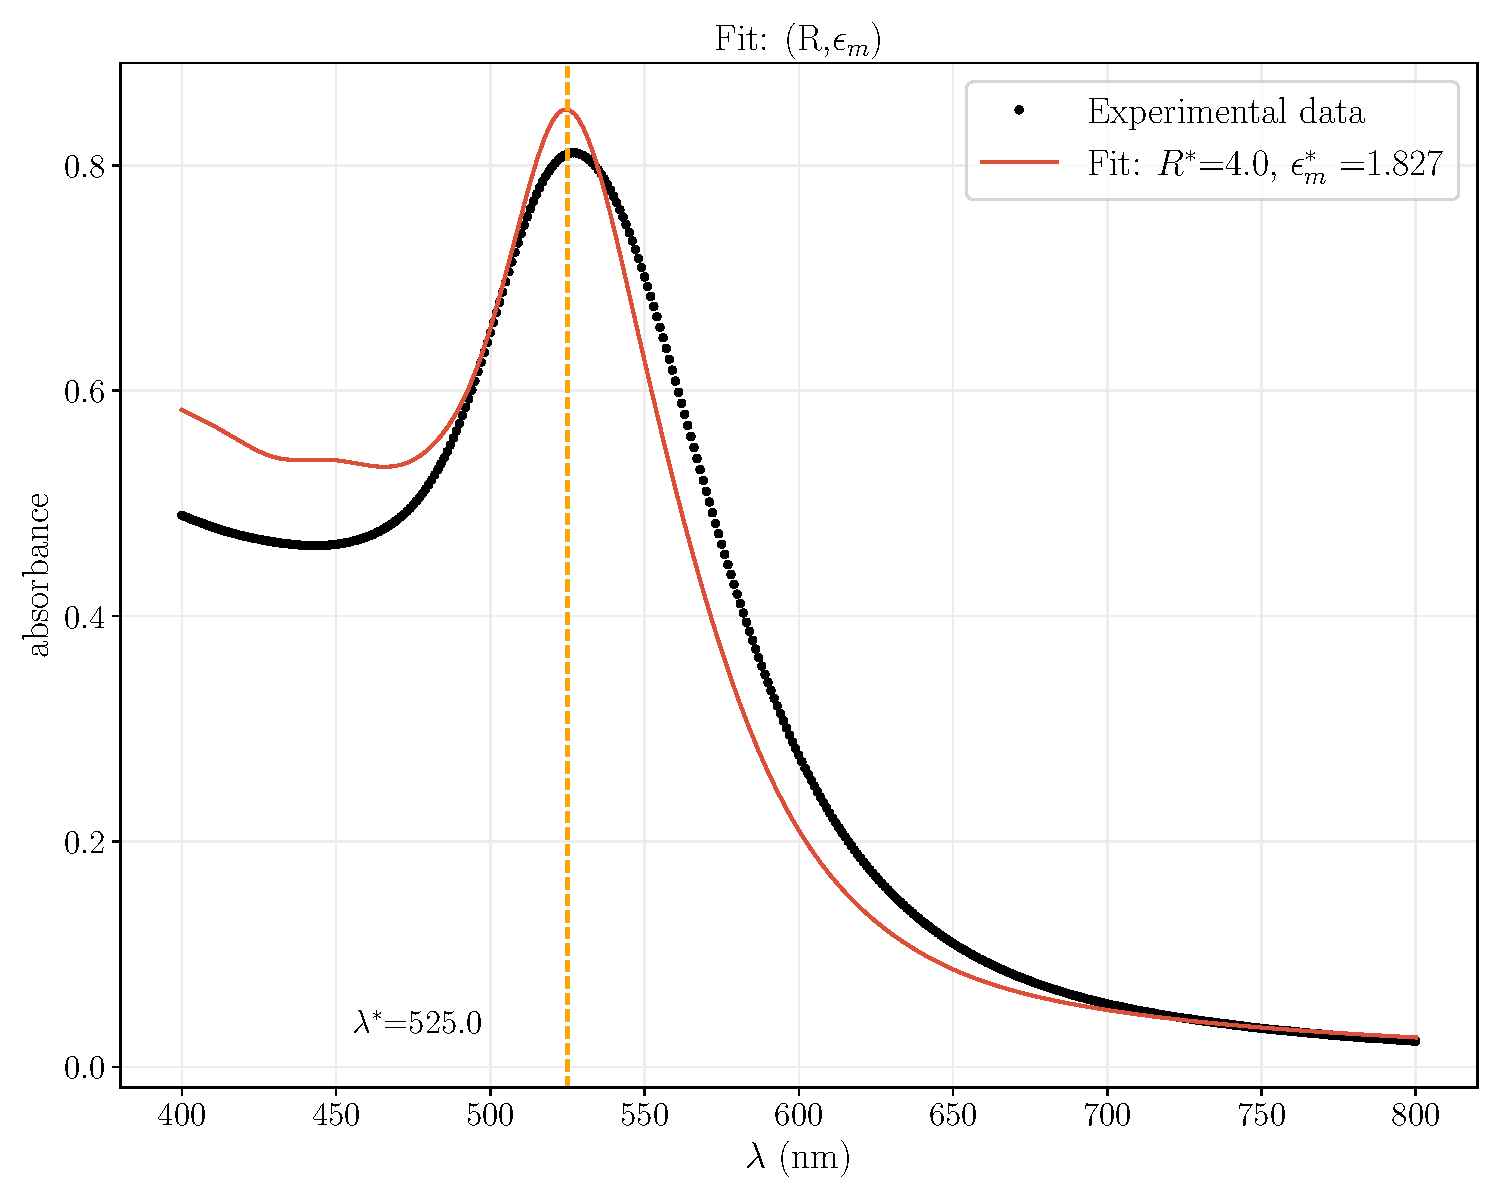
\includegraphics[width=.5\textwidth]{image/data/2_fit.pdf}} 
\subfloat[][{Map of the $\chi^2$ function for ($R,\epsilon_m$).}]
{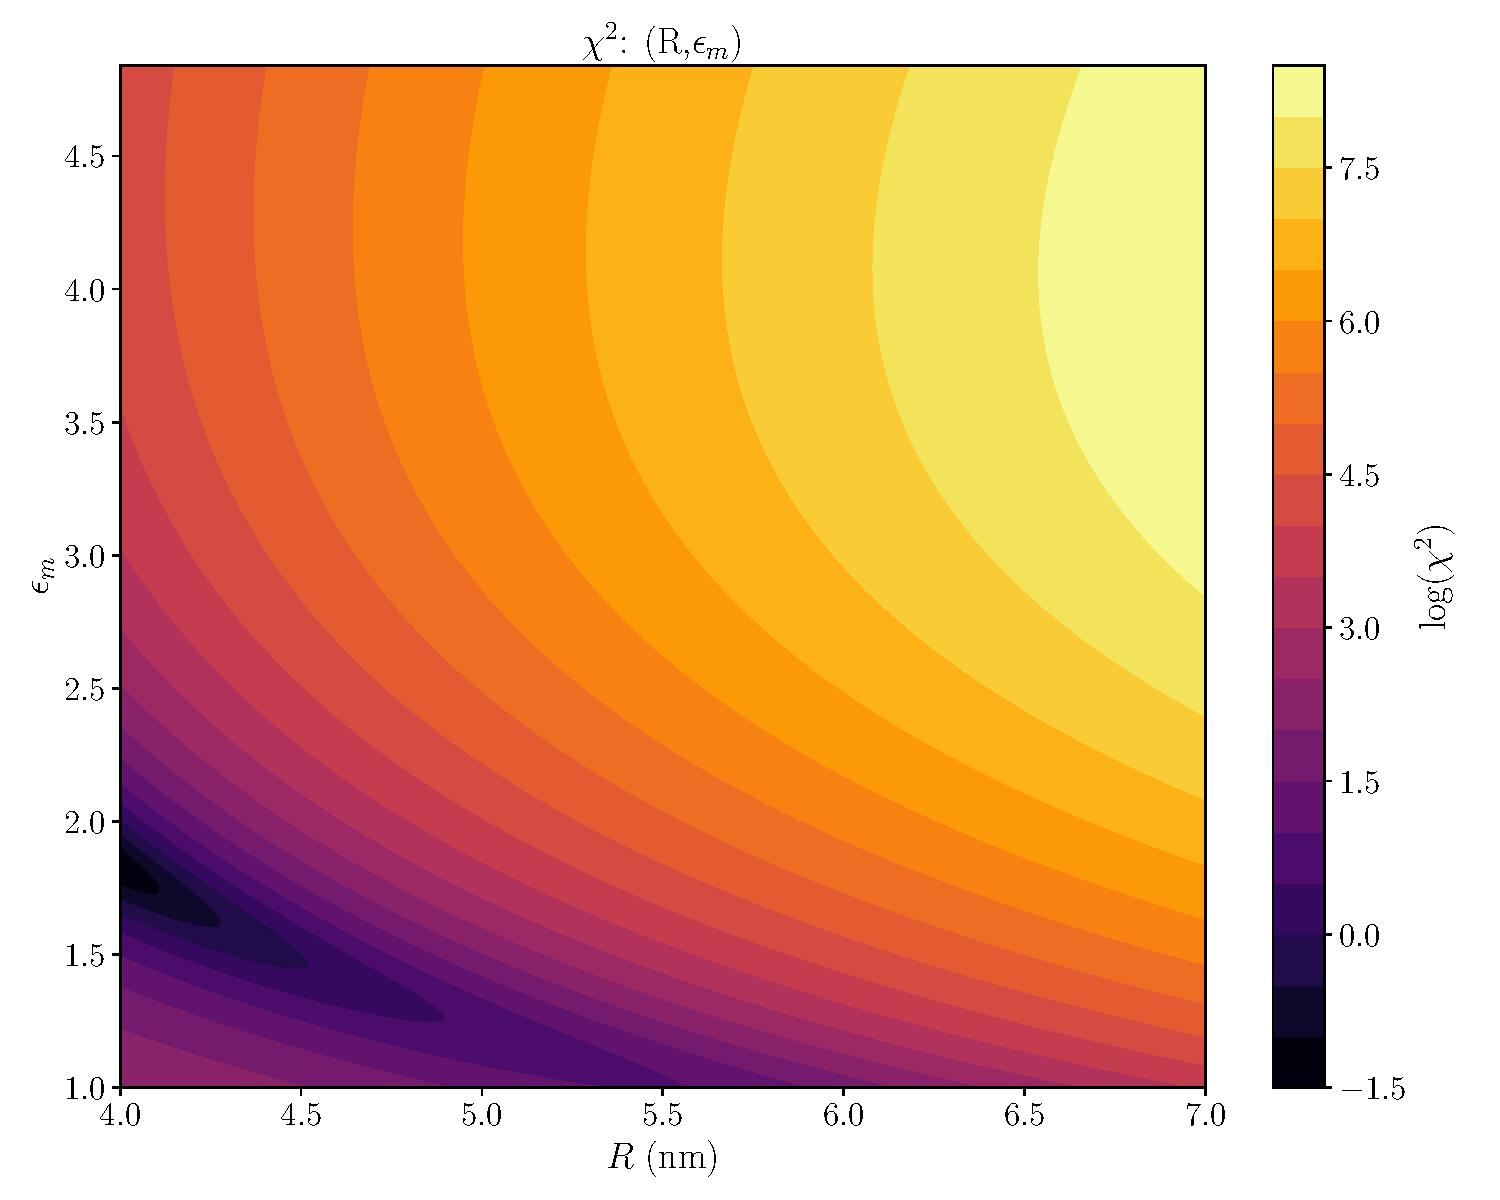
\includegraphics[width=.5\textwidth]{image/data/2_chisquare.pdf}} \\
\caption{Simulation, fit and plot of the $\chi^2$ function for the ($R,\epsilon_m$) couple.}
\label{fig:r_epsm}
\end{figure}
\newpage

\begin{multicols}{2}
In the end, despite of the fact that the particles' radius is less then 20 times smaller than the incoming wavelength (which proves the validity of the $R\ll \lambda$ hypothesis), the computations reported in this section have been performed  using the dipolar approximation only: this model could have been improved by taking into account higher multipolarities.

\subsubsection{Gans' Model Analysis}
\paragraph{Model}
The results presented in \textbf{Section \ref{sec:risultati}} can be improved by refining the model used in this analysis by means of the Gans' theory (instead of the Mie's one).

Gans' theory considers nanoparticles to be oblate ellipsoids\footnote{In this way it's possible to drop the spherical Au nanoparticles assumption.} introducing a new parameter $e$ called eccentricity.

\noindent
The new model computes the extinction cross-section as an ensemble of ellipsoidal particles with spatial random orientation \cite{mattei}:

\begin{equation*}
\sigma_{ext}^{\text{Gans}} = \frac{\omega}{3c} \epsilon_m^{3/2}V_{0} \sum^{3}_{j=1}{\frac{\epsilon_2/L_j^2}{[\epsilon_1 + \epsilon_m(1-L_j)/L_j]^2 + (\epsilon_2)^2}}
\end{equation*}

\noindent
where $V_0$ is the volume of the ellipsoid and the $L_{j,j=\{1,2,3\}}$ parameters are called polarization coefficients:
\begin{align*}
L_{1}&=\frac{1-e^{2}}{e^{2}}\left[\frac{1}{2 e} \ln \left(\frac{1+e}{1-e}\right)-1\right]\\
L_{2}&=L_{3}=\frac{1-L_{1}}{2}
\end{align*}

\paragraph{Results}
Given the data presented in \textbf{Section \ref{sec:SEM}} (i.e. the average of the major
and minor axis of the two dimensional representation of the particles $a_1$ and $a_2$\footnote{We assumed that the third axis $a_3=a_2$, s.t. $a_1>a_2=a_3$.}) we were able to estimate the aspect ratio $a_R$ as  $a_1/a_2$ resulting in:

\[a_R=1.30\pm 0.01\]

At this point we were able to compute\footnote{The error associated to estimated measurement of the eccentricity has been computed by means of the propagation of errors.} the eccentricity $e$ and to use Gans' model, namely:

\[e:=\sqrt{1-\left(\frac{1}{a_R}\right)^2} = 0.638 \pm 0.007\]

We can notice from \textbf{Figure \ref{fig:r_rho_GANS}a} and \textbf{Figure \ref{fig:r_epsm_GANS}a } that the fit quality is slightly improved with respect to the plots shown in \textbf{Figure \ref{fig:r_epsm}a} and \textbf{Figure \ref{fig:r_epsm}a}. In particular, the experimental values of absorbance in the lower frequency range ($\lambda \in [400:475]\, \nano\meter$) are better represented by the simulation with respect to the ones in \textbf{Section \ref{sec:risultati}}.

The better agreement between the experimental spectrum and the model may be due  to the fact that ellipsoidal particle give a different position of the resonance for each length of the axis and so the width of the peak can be better covered by the two resonances of our model. \textbf{Figure \ref{fig:r_rho_GANS}b} and \textbf{Figure \ref{fig:r_epsm_GANS}b} show the $\chi^2$ map  for the ($R,\rho$) and ($R,\epsilon_m$) couple of parameters respectively.

After performing the Gans analysis, the parameters which describe better our physical system are:

\begin{align*}
    R^*_{G}&=(6.4\pm 0.9)\,\nano\meter \\
    \rho^*_{G}&=(2.0\pm 0.3)\cdot 10^{-9}\,\nano\meter^{-3} \\
    \epsilon_{m,G}^* &= 1.9 \pm 0.1
\end{align*}
As the value of $R^*_G$ increased with respect to $R^*$, consequently the value of $\rho_G^*$ is lower than $\rho^*$.

In the end, we can notice that the best value of $\epsilon_m$ improved: $\sqrt{\epsilon_{m,G} ^*} := n_{water,G}^*$ differs from the true value $n_{water}=1.33$ by $4\%$.

\end{multicols}
\newpage
\begin{figure}[H]
\centering
\subfloat[][{Simulated spectrum obtained by varying the parameters ($R,\rho$) and fit with the experimental data using Gans' theory.}]
{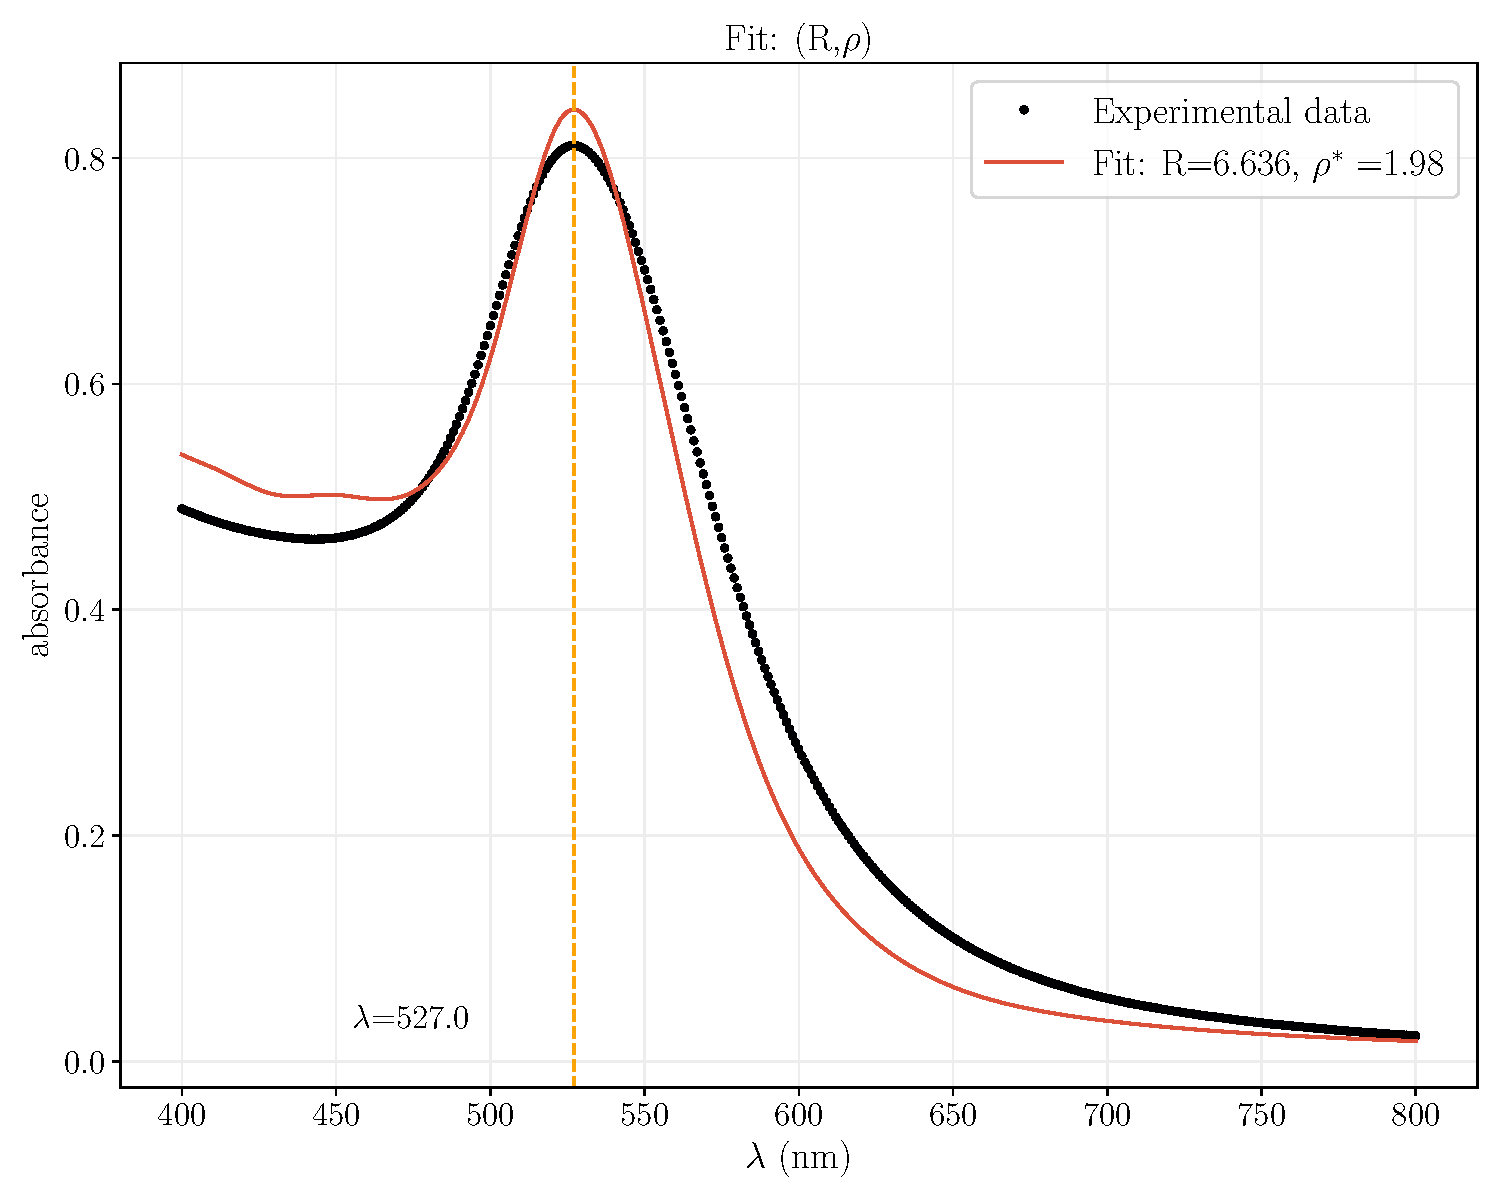
\includegraphics[width=.5\textwidth]{image/data/1_fit_GANS.pdf}} 
\subfloat[][{$\chi^2$ function for ($R,\rho$) using Gans' theory.}]
{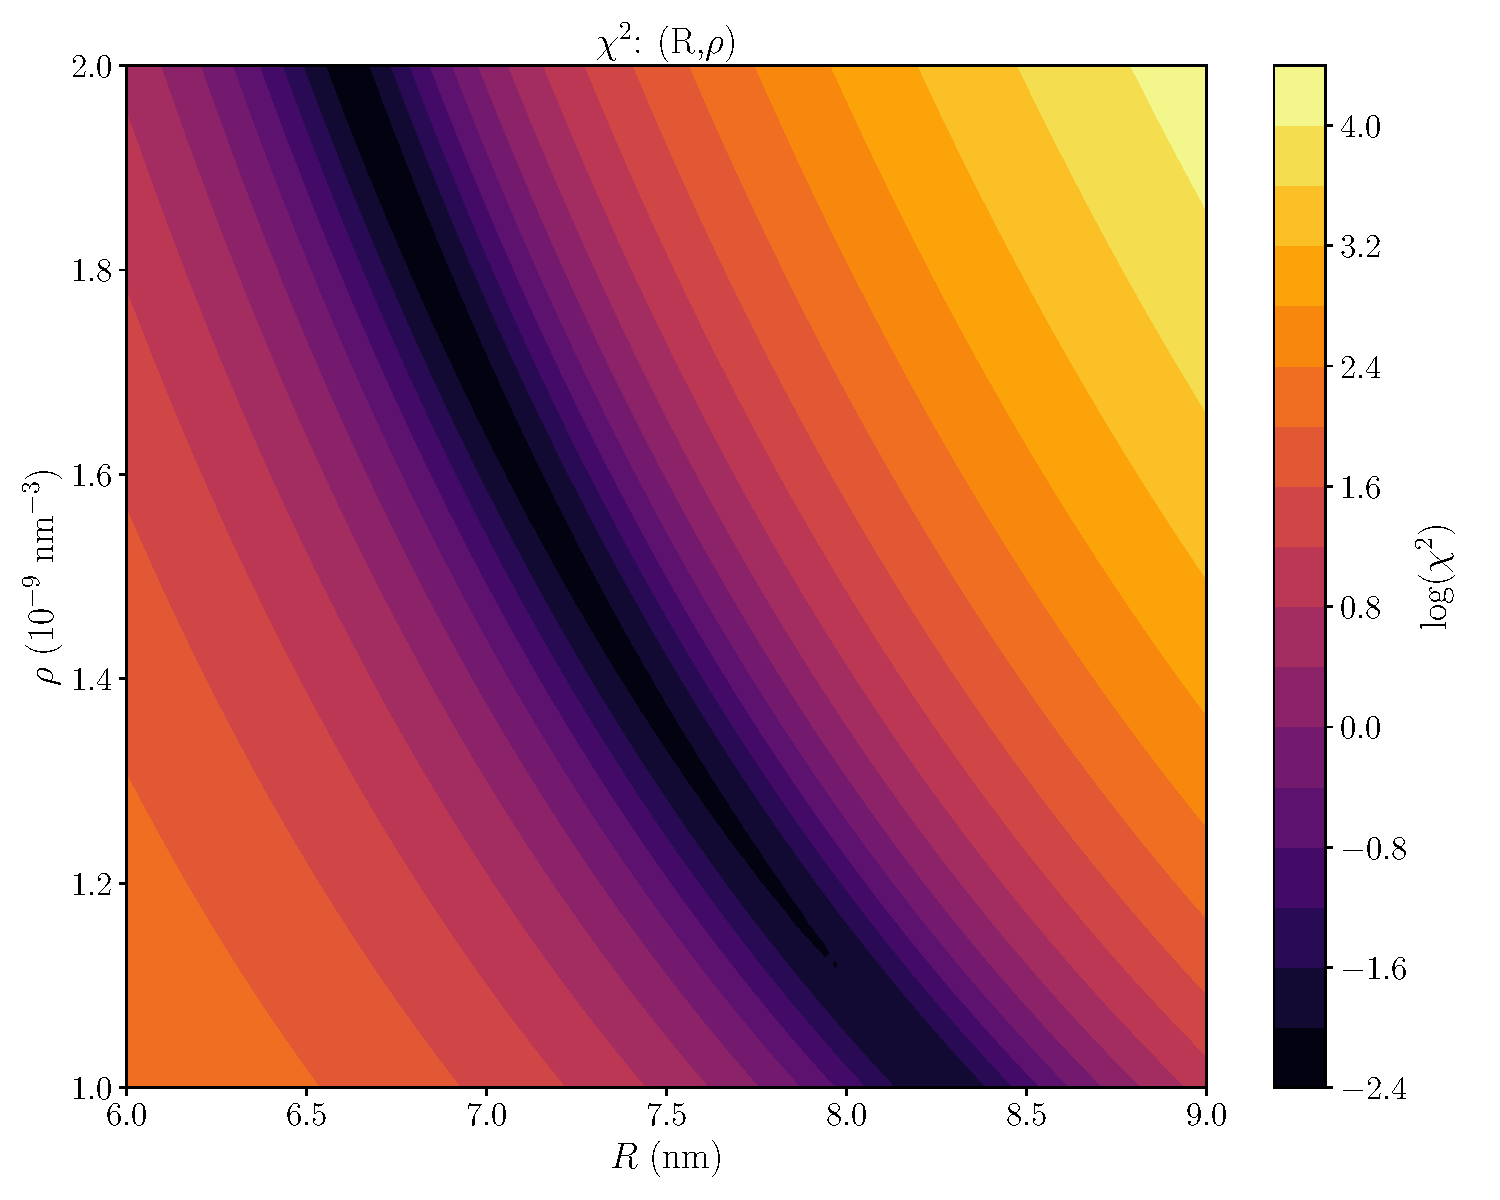
\includegraphics[width=.5\textwidth]{image/data/1_chisquare_GANS.pdf}} \\
\caption{Simulation, fit and plot of the $\chi^2$ function for the ($R,\rho$) couple using Gans' theory.}
\label{fig:r_rho_GANS}
\end{figure}

\begin{figure}[H]
\centering
\subfloat[][{Simulated spectrum obtained by varying the parameters ($R,\epsilon_m$) and fit with the experimental data using Gans' theory.}]
{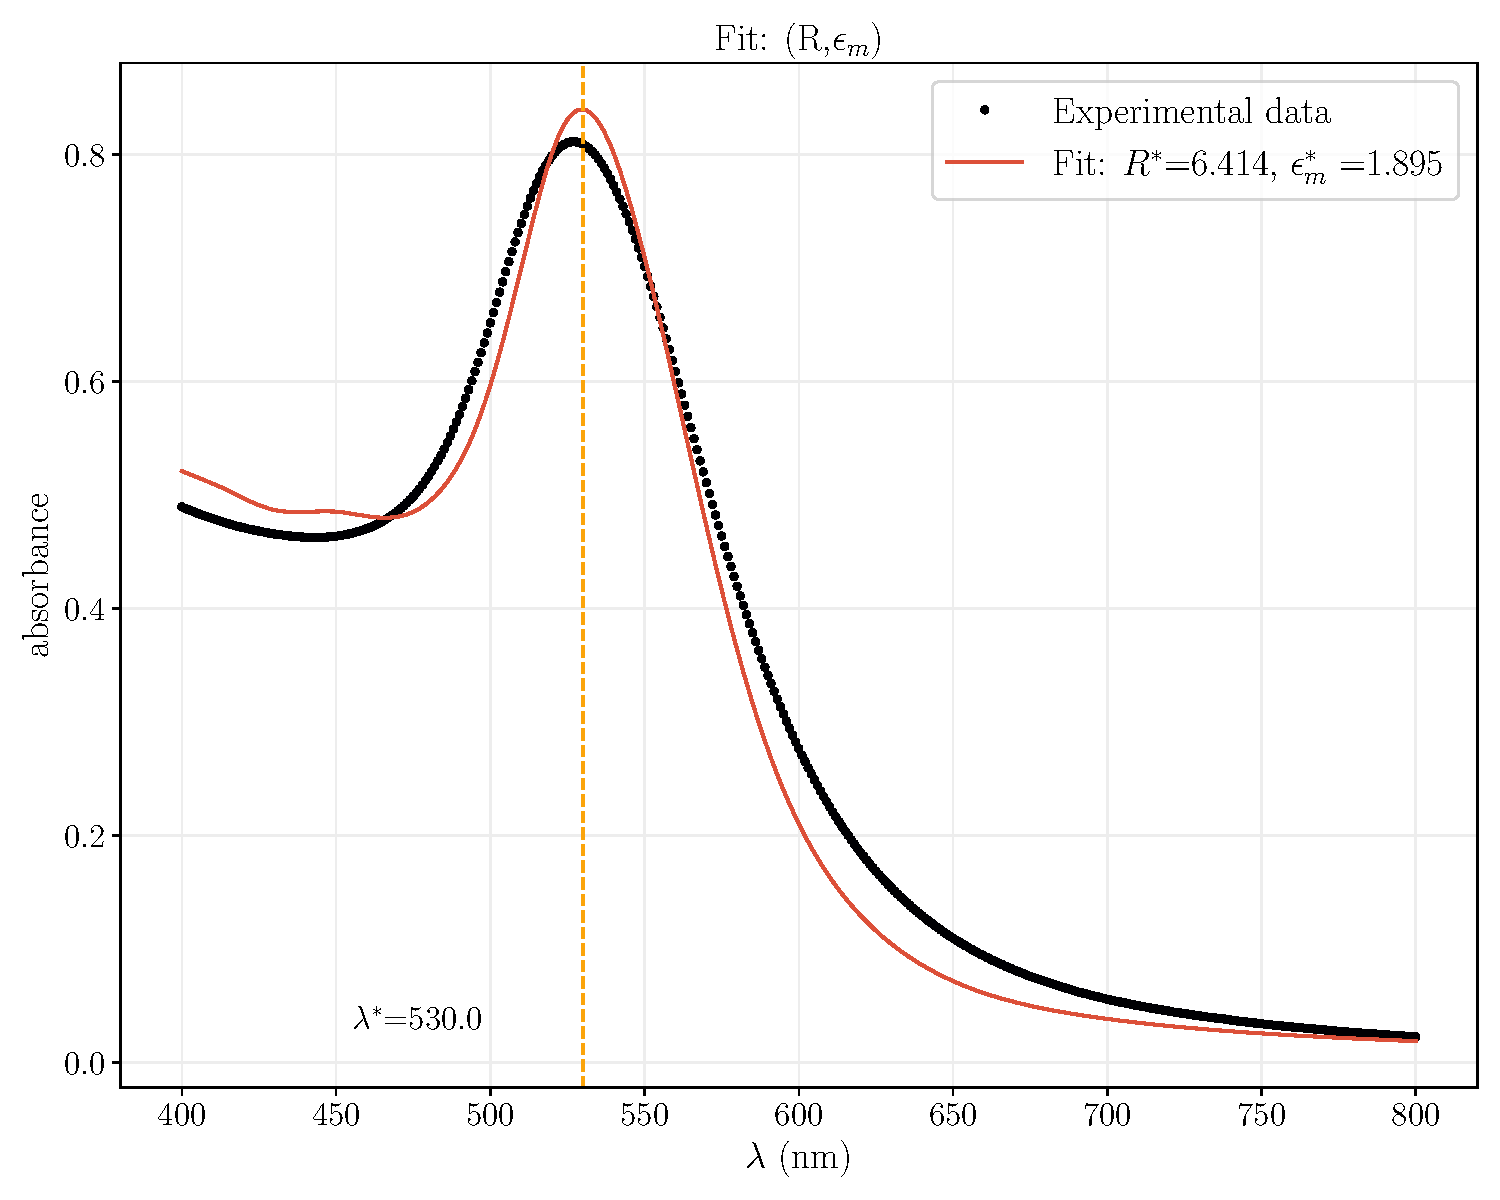
\includegraphics[width=.5\textwidth]{image/data/2_fit_GANS.pdf}} 
\subfloat[][{$\chi^2$ function for ($R,\epsilon_m$) using Gans' theory.}]
{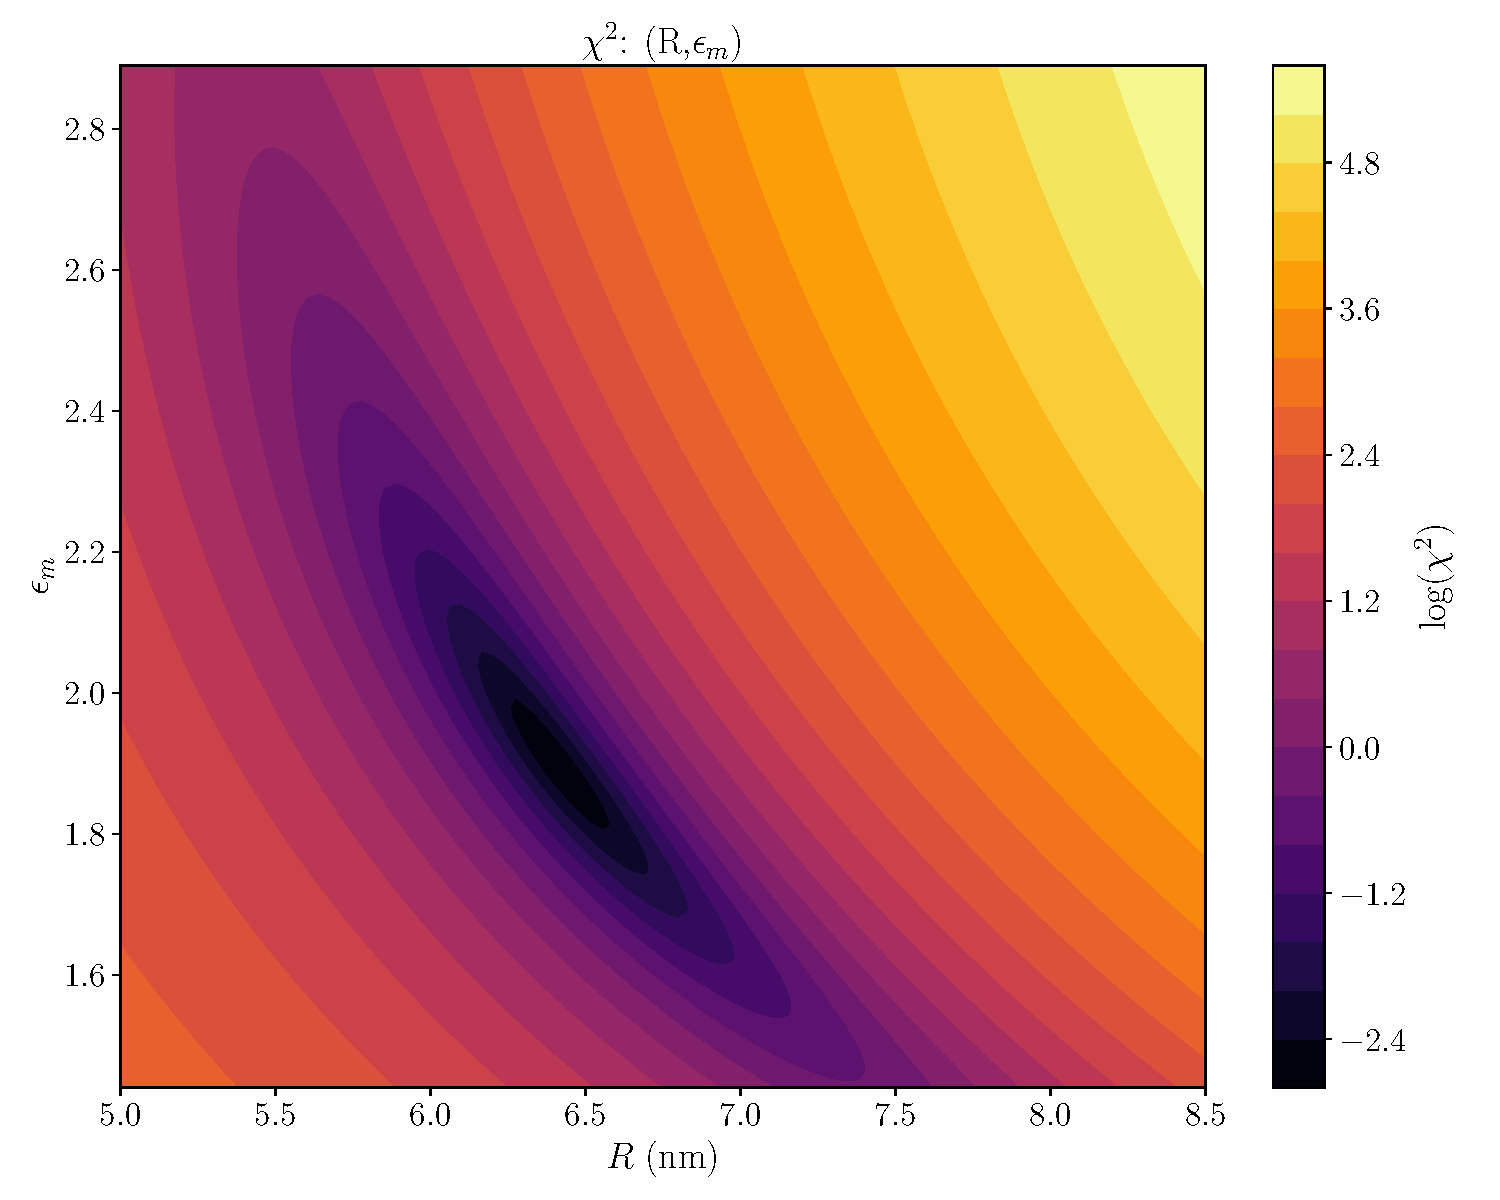
\includegraphics[width=.5\textwidth]{image/data/2_chisquare_GANS.pdf}} \\
\caption{Simulation, fit and plot of the $\chi^2$ function for the ($R,\epsilon_m$) couple using Gans' theory.}
\label{fig:r_epsm_GANS}
\end{figure}
\newpage

\begin{multicols}{2}

\section{XRD Analysis}

\label{sec:XRD}

\subsection{Method}

\subsection{Results}

\section{SEM Analysis}
\label{sec:SEM}

\subsection{Imaging with SEM}
\label{sec:synthesis}
\noindent
Nano-sized images of the gold nanoparticles in the silicon substrate were collected using a Scanning Electron Microscope (SEM) which exploits the emission of secondary and backscattering electrons to generate the image.

The image shown in \textbf{Figure \ref{fig:semss}} was used to perform a measurement of the area, major axis and minor axis of the nanoparticles, assuming that their projection on the image plane is elliptical.

\begin{figure}[H]
    \centering
    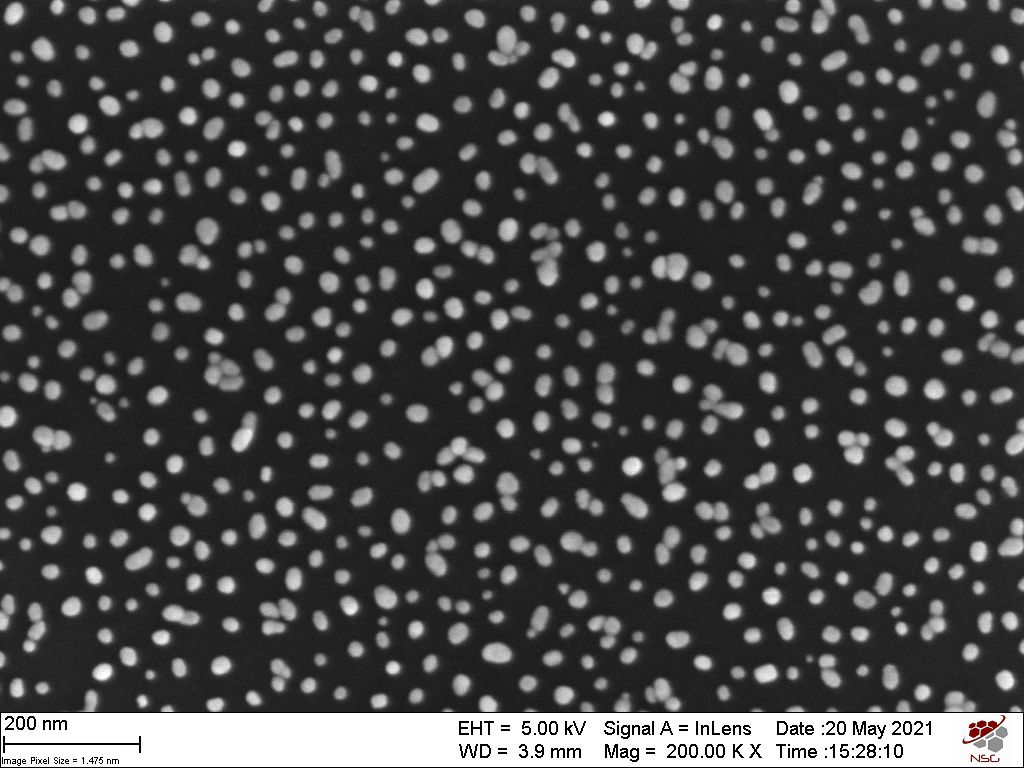
\includegraphics[width=\linewidth]{image/data/imaging.jpg}
    \caption{Imaging obtained with SEM.}
    \label{fig:semss}
\end{figure}

After obtaining this image, ImageJ software was used to extract the required data. Groups of nanoparticles that failed to distinguish as individual particles were excluded from subsequent measurements. Two pixels have been chosen as the maximum error on the lengths, which is then converted into nanometers and used for the calculation of subsequent values.
Subsequently, the effective diameter of the nanoparticle was obtained from the area value of the i-th particle using the following equation:
\begin{align*}
D_{eff,i}=2\sqrt\frac{A_{i}}{\pi}
\end{align*}

where $A_i$ is the area of the i-th particle and $D_{eff,i}$ is the effective diameter of i-th particle. Notice that the error on the single diameter will depend on the value of the area and its i-th error using propagation of errors equation.

In conclusion it was calculated the aspect ratio of i-th particle as the ratio of major axis to minor axis:
\begin{align*}
a_{R,i}=\frac{a_{1,i}}{a_{2,i}}
\end{align*}

\subsection{Results}
After having calculated all the effective diameters, an histogram of the nanoparticles' diameters distribution is constructed and is then fitted with a lognormal distribution that gives us the most frequent value of the diameter of the nanoparticles and its dispersion.

\begin{figure}[H]
    \centering
    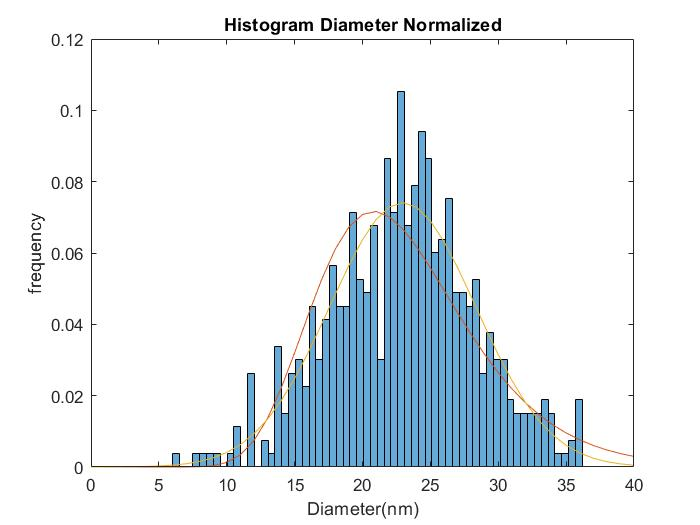
\includegraphics[width=\linewidth]{image/data/fitlognorm.jpg}
    \caption{Histogram of diameter normalized at probability distribution function. Red: Lognormal fit. Yellow: Gaussian fit.}
    \label{fig:diameter_distribution}
\end{figure}

\gio{secondo me sarebbe carino vedere anche le labels delle figure, in particolare per figura 9. Secondo me i due fit non si vedono bene, forse sarebbe meglio ingrandirli}

The fit lognormal results give us the following diameter:
\begin{align*}
\mean{D}=(22 \pm 1) \, \nano\meter
\end{align*}

Then $\sqrt[3]{\mean{D^3}}$ was calculated using the formula of the average, weighted with the errors of the single diameter, the result of which leads to:

\begin{align*}
\sqrt[3]{\mean{D^3}}=(21.3 \pm 0.3) \, \nano\meter
\end{align*}

Comparing the two diameters with the compatibility test:
\begin{align*}
\lambda=\frac{|\sqrt[3]{\mean{D^3}}-\mean{D}|}{\sqrt{\sigma_{\mean{D^{3}}}^{2}+\sigma_{\mean{D}}^{2}}}\approx0.7
\end{align*}

\noindent
where $\sigma_{\mean{D^3}}$ is the error of $\sqrt[3]{\mean{D^3}}$. The value 0.7 corresponds to an optimal compatibility.

The aspect ratio is also calculated by simply exploiting the average. The result obtained is:
\[a_R=1.30\pm 0.01\]
This value was also used in \textbf{Section 3.2.1} for the correction, using Gans theory, of the radius value obtained with the minimum chi squared. 

In conclusion, the distribution of the aspect ratios is shown for completeness:
\begin{figure}[H]
    \centering
    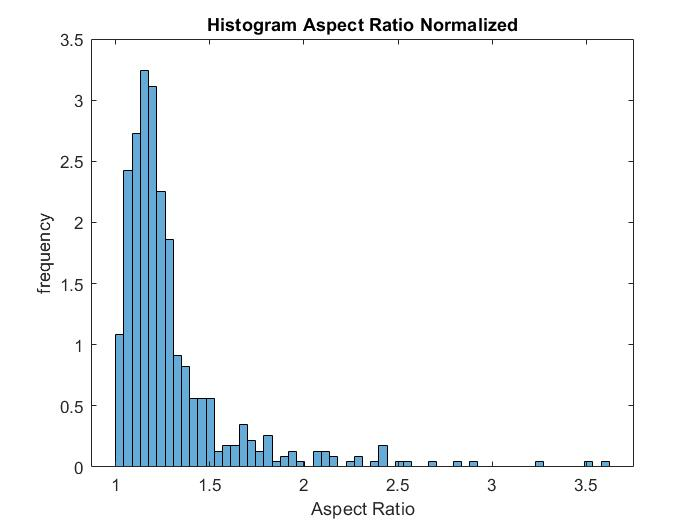
\includegraphics[width=\linewidth]{image/data/a_r distribution.jpg}
    \caption{Histogram of aspect ratio normalized at probability distribution function.}
    \label{fig:aspect_ratio}
\end{figure}


\section{Conclusions}
\label{sec:conclusions}
We characterized the gold nanoparticles using three different methods: Optical Spectroscopy, X-rays and Scanning Electron Microscopy.

For every method we computed the average size of the synthesized nanoparticles. The results of our work all agree on the order of magnitude of the nanoparticles' radii but their values (presented in \textbf{Table \ref{sec:risultati}}) are quite different, making our estimates incompatible with each other.

Concerning the optical analysis, the hypothesis assumed in \textbf{Section \ref{sec:optic_char}} are quite strong and in particular considering the nanoparticles' shape as spherical. For this reason the value of the radius obtained using Gans' theory ($R^*_{G}$) improves the result of the Mie theory analysis, making it possible to approach the value of $\mean{R}$ obtained by the SEM analysis (which we consider to be the reliable measure among the three methods). 

If the radii of the previous sections are compared with the radius obtained using the measurement with the SEM it is clear that there is an enormous difference between the values obtained which makes them incompatible. The first explanation could be due to the inaccuracy of the correction of \[\Gamma(R)=\Gamma_{bulk}+k \frac{v_{F}}{R}\] as the second contribution was calculated assuming the spherical nanoparticles (da capire). The second explanation ....

\gio{sarebbe bello aggiungere una tabellina finale con i tre valori dei raggi che abbiamo trovato}

\begin{table}[H]
    \centering
    \caption{Values of the characteristic length of the nanoparticles obtained using the three different methods presented in this work.
    \gio{L'errore è lo stesso perché considero l'errore come la sigma della distribuzione lognormale che non cambia se moltiplico per 2 ogni valore}}
    \begin{tabular}{cccc}
    \toprule
      & \textbf{GANS}\,(\nano\meter)   & \textbf{XRD}\,(\nano\meter)  & \textbf{SEM}\,(\nano\meter)  \\
    \midrule
     $\mean{R}$ & $6.4\pm 0.9 $   & $?? \pm ?$ & $11 \pm 1$ \\
    \bottomrule
    \end{tabular}
    \label{tab:results}
\end{table}

\clearpage
\end{multicols}
\printbibliography


\end{document}